\documentclass {beamer}
\usepackage{graphicx} % Required for inserting images


\title{UYKU PUANLAMASINA İSTATİSTİKSEL BİR BAKIŞ}
\author{Okan Bahadır Soygür}
\subtitle{İST480 Araştırma Yöntemleri}
\date{Haziran 2023}

 \logo{
\includegraphics[scale=0.04]{logo.png}}

\usetheme{CambridgeUS}



\begin{document}

\maketitle

\section{Makalenin Yayınlandığı Dergi Ve Makale Hakkında Genel Bilgiler}
\begin{figure}[h]
    \centering
    
\includegraphics[width=0.80\linewidth]{aüff.png}
    \label{fig:enter-label}
\end{figure}
\textbf{Dergi Adı:}  Communications Faculty of Sciences University of Ankara Series A2-A3: Physical Sciences and Engineering.


\textbf{Dergi İndeksi:} TrDizin, DergiPark

\textbf{Dergi Hakkında:} Communications Faculty of Sciences University of Ankara Series A2-A3: Physical Sciences and Engineering dergisi, 1948 yılında yayım hayatına İngilizce olarak başlamış ve bu tarihten itibaren sadece İngilizce hazırlanan makaleleri yayımlayarak devam eden hakemli ve açık erişimli dergidir. Ankara Üniversitesi Fen Fakültesi tarafından yayımlanan, Fizik, Elektronik/Bilgisayar Mühendisliği, Astroloji ve

Jeofizik adanan bu dergi 1994 yılından itibaren yayımlanan 


sayılarla birlikte TrDizin tarafından indekslenmeye başlamıştır. 

Dergi Haziran ve Aralık olmak üzere yılda 2 sayı yayımlamaktadır 


ve okurlarından herhangi bir ücret talep etmemektedir.



\textbf{Derginin Erişim Linki:} http://communications.science.ankara.edu.tr/?series=A2A3

 \begin{frame}
 \textbf{Makale Adı:} A Statistical Overview On Sleep Scoring
 \textbf{Yazarlar:} Levent ÖZBEK, Levent SÜTÇİGİL, Hamdullah AYDIN, Sinan YETKİN, Fuat ÖZGEN
 
 \textbf{Makale Dili:} İngilizce
 
 \textbf{Makalenin Konusu:} İstatistiksel modellemede sıklıkla kullanılan uyku EEG'si otoregresif (AR) zaman serisi modeli ile modellenmiş ve farklı uyku evrelerinde temsil edilen modelde yer alan beyaz gürültü teriminin varyansının nasıl bir yapı olduğunun incelenmesi.


 
 \textbf{Makalenin Amacı:} Rechtschaffen ve Kales kriterlerine göre puanlanan tüm aşamalar ayrı ayrı dikkate alınarak her aşamadaki dönemler AR ile modellenip bu modelde beyaz gürültü terimi varyansının izlenmesi.
 
\textbf{Makalenin Önemi:} Uyku skorlaması, uyku örüntülerinin 


araştırılmasında hastalıkların sınıflandırılması ve uygun tedavi 


uygulamaları için önemli bir adımdır. Şu anda Rechtschaffen ve 

Kales sınıflandırması geçerlidir.

    
 \end{frame}


\begin{frame}{Makalenin Metadolojisi}

\textbf{Örnekleme Planı:}
\begin{itemize}
    \item Kitle: Genç ve Sağlıklı psikiyatrik şikayeti olmayan denekler.

    \item Örneklem:Herhangi bir psikiyatrik şikayeti olmayan denekler GATA Ruh Sağlığı ve Hastalıkları Daire Başkanlığı Uyku Araştırmaları Merkezi'nde iki gece süreyle çalışma hakkında bilgilendirilerek polisomnografik incelemeye alınmıştır.
\end{itemize}

\textbf{Veri Toplama Yöntemi}:Somnostar Alpha adlı polisomnograf kullanılmıştır.

\textbf{Veri Toplama Süresi:} Polisomnografik incelemelerin her biri otuz 

saniye süren dönemler halinde puanlanıp EEG kaydı (C3-A2) 

ikinci gece değerlendirmeye alınır.

\textbf{Uygulanan Yöntemler:} Polisomnografik muayene.
\end{frame}
 
\begin{frame}

\begin{figure}1
    \centering
    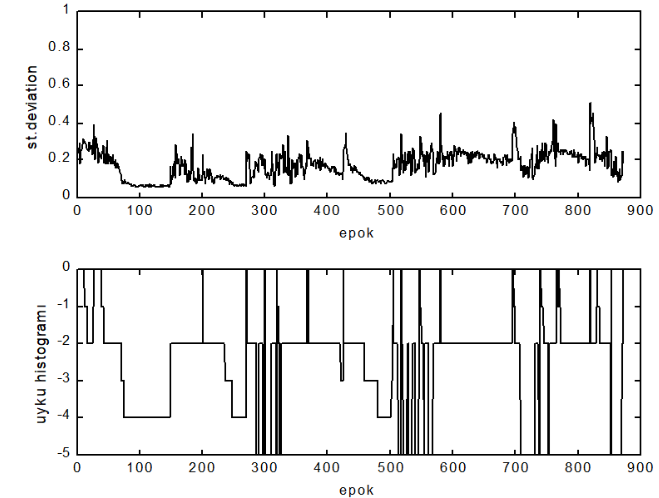
\includegraphics[width=0.75\linewidth]{figure1.png}
    \caption{Uyku histogramı ve standart sapmalar}
    \label{fig:enter-label}
\end{figure}
\end{frame}

\begin{frame}
\begin{figure}2
    \centering
    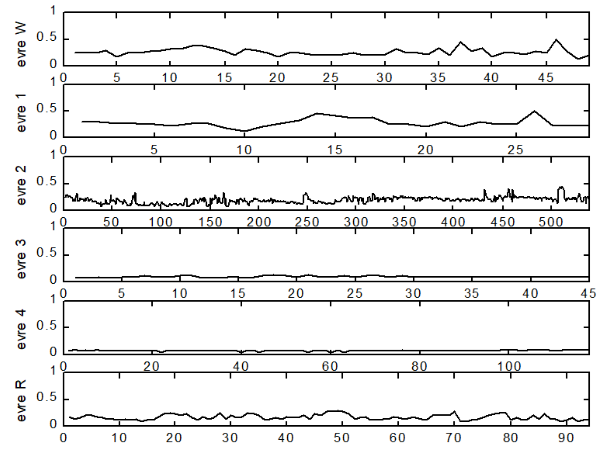
\includegraphics[width=0.75\linewidth]{figure2.png}
    \caption{Aşamalara göre standart sapmalar}
    \label{fig:enter-label}
\end{figure}
\end{frame}

\begin{frame}
\textbf{Sonuç ve Tartışma:}
Çalışma, bir öznenin uyku EEG varyanslarını değerlendirmiştir. Şekil 2'de verilen sonuçlara göre, puanlamada objektif farklılıkların ortaya çıkmasının 2. Aşamadaki heterojenlikten kaynaklandığı düşünülmüştür. Bu verilerin, Aşama 2 olarak adlandırılan Rechtschaffen ve Kales puanlamasındaki dönemin yeniden gözden geçirilmesi gerekliliğine işaret ettiği düşünülmektedir.
\end{frame}

\begin{frame}{Makale Hakkında Görüşler}

\textbf{Makalenin artı yönleri:}
\begin{itemize}
    \item Bu makale, 20.yy'dan itibaren kullanılan temel elektrofizyolojik yöntemlere dayalı uyku çalışmaları sayesinde yazılmıştır.
    \item Örneklem büyüklüğü yeterlidir.
    
\end{itemize}

\textbf{Makalenin eksi yönleri:}
\begin{itemize}
    \item Modellerde kullanılan değişkenler yetersizdir. 
\end{itemize}
\end{frame}
\begin{frame}{Kaynakça}
\begin{enumerate}
    \item Berger, H., Ueber das Elektroenkephalogramm des Menschen, J. Psychol. Neurol, 40 
(1930), 160-179. 
\item Aserinsky, E., Kleitman, N., Regularly occuring periods of eye motility and 
concomitant phenomena  during sleep, Science, 118 (1953), 273-274. https://doi.org/ 
10.1016/j.jqsrt.2012.05.012. 
\item Dement, W., Kleitman, N., Cyclic variations in EEG during sleep and their relation to 
eye movements, body motility and dreaming, EEG Clin. Neurophysiol., 9 (1957), 673-
690.  
\item Rechtschaffen, A., Kales, A., A manual of Standized Therminology Techniques and 
Scoring  System  for  Sleep  Stages  of  Human  

Subjects, 
Brain  Information  Service/ 
Brain Research Institute, University

of California, Los Angeles, 1968. 
\item Bazil, C.W., Castro, L.H., Walczak, T.S., Reduction of rapid

eye movement sleep by 
diurnal  and  nocturnal  seizures  in  

temporal  lobe  epilepsy,  Arch.  Neurol.  57  (2000), 
363-368. 

\end{enumerate}



\end{frame}
\end{document}


